\documentclass{article}

\usepackage[utf8]{inputenc}
\usepackage[french]{babel}
\usepackage{amsmath}
\usepackage{graphicx}
\usepackage{amssymb}

\title{COMPTE-RENDU TP3}
\author{ISIK Umut,\\ NAIT-DAOUD Mohamed,\\ Université Paris 13,\\ L2-Mathématiques,\\ Maths AP,}

\begin{document}

\maketitle

\section{Introduction}

En tant qu'étudiant en mathématiques nous allons être confronté, durant notre formation, à la résolution de problèmes à partir d'outils informatiques. Afin de nous familiariser avec ceux-ci on étudiera les méthodes pour intégrer numériquement sur un intervalle $ t \in [0,T] $, une équation différentielle ordinaire (EDO) c'est-à-dire de la forme : $$ u^{'}(t)=f(t,u(t)), ~~ u(0)=u_{0} $$

\section{Exemple d'EDO}

Soit l'EDO $ u^{'}(t) = -u(t), ~~ u(0)=1.0 $.\\
Ici la fonction f est $\exp(-t)$.

\begin{align*}
u^{'}(t)= -u(t) &\iff \frac{u^{'}(t)}{u(t)} = -1 \\
				&\iff \ln(u(t))^{'} = -1 \\
				&\iff \ln(u(t)) = \int -1 ~\mathrm{d}t \\
				&\iff \ln(u(t)) = -t+C_1 && C_1 \in C^{n}(\mathbb{K},\mathbb{K}) \\
				&\iff u(t) = e^{C_1}e^{-t} \\
\end{align*}
On va déterminer la constante à partir des conditions initiales.\\ On sait que ~~ $u(0)=1.0$ et $u(0)=e^{C_1}e^{0}$.\\
On a alors $e^{C_1}=1.0$ donc $C_1=0$.\\
Donc la solution de cette EDO est $u(t)=e^{-t}$
\begin{center}
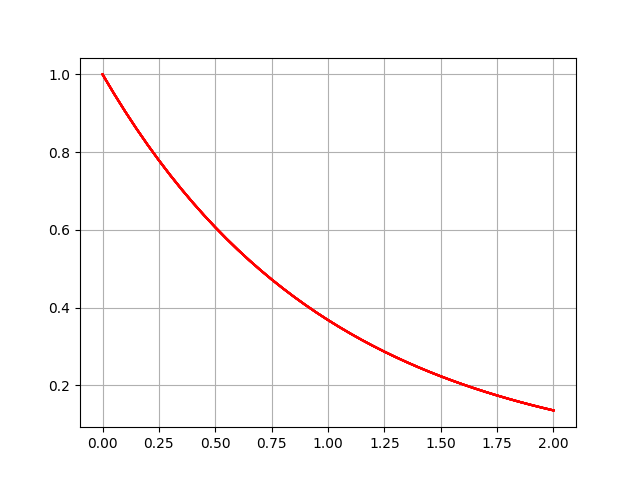
\includegraphics[scale=0.5]{fig1.png}
\end{center}

\section{Calcul à partir de la méthode d'Euler}

On a utilisé la méthode d'Euler pour calculer les onze premiers termes de la suite $(u_{k})$, définie par la méthode d'Euler.
\begin{center}
\begin{tabular}{|c|c|c|c|c|}

\hline
$u_{1}=0.8 $& $u_{2}=0.64 $& $u_{3}=0.512$ &$ u_{4}=0.4096 $& $u_{5}=0.32768 $\\
\hline
$u_{6}=0.262144 $&$ u_{7}=0.2097152 $& $u_{8}=0.16777216$ &$ u_{9}=0.13421773$ &$ u_{10}=0.10737418 $\\
\hline

\end{tabular}
\end{center}

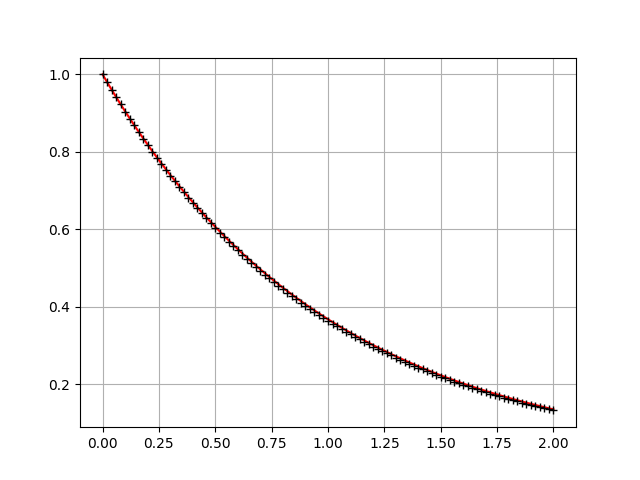
\includegraphics[scale=0.5]{graphexo2.png}
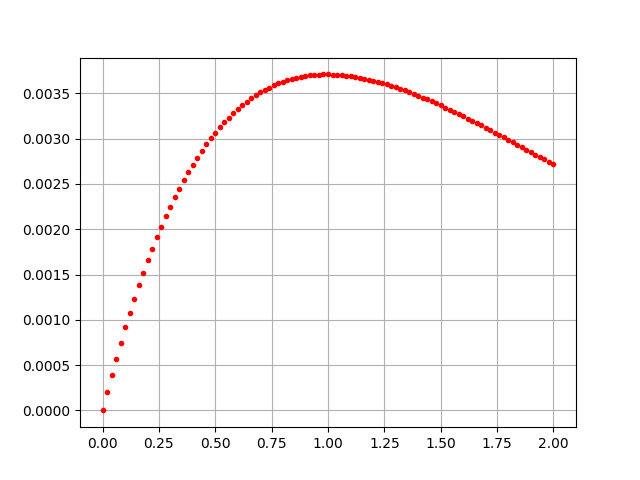
\includegraphics[scale=0.5]{erreur_exo2.png}\\

Le graphique à gauche montre l'approximation de la solution de l'EDO à partir de la suite $(u_k)$. On remarque qu'en prenant un petit nombre d'éléments de $(u_k)$ l'erreur d'approximation s'accroit puis tend à se confondre avec la solution car la solution et la suite tendent vers $0$ en $+\infty$. Ainsi la méthode d'Euler sera d'autant plus efficace et pécise quon prendrai d'éléments de $(u_k)$.

\section{Fonction Euler}

On a écrit une fonction python euler et on l'a appliquée à l'exemple précedent. On a obtenu les mêmes résultats.
On a ensuite étudié trois autres EDO :
\begin{equation}
u^{'}(t)=-u(t)+t ~~ u(0)=1.0
\end{equation}
\begin{equation}
u^{'}(t)=u^{2}(t) ~~ u(0)=1.0 
\end{equation}
\begin{equation}
u^{'}(t)=u^{2}(t)-t ~~ u(0)=1.0 
\end{equation}

L'EDO (1) est une équation différentielle linéaire du premier ordre. On doit d'abord trouver la solution de l'équation homogène puis la solution particulière. La solution de l'équation sera la somme des deux.\\

On sait que la solution de l'équation homogène est $ X(t)=e^{-t}$.\\
Pour la solution particulière, on sait que la solution est de la même forme que le second membre de l'équation alors $Y(t)=At$ avec $A\in C^{n}(\mathbb{K},\mathbb{K})$\\
$A+At=t \iff A(1+t)=t \iff A=\frac{t}{1+t}$ \\
Alors on a $Y(t)=\frac{t^2}{1+t}$.\\
Donc la solution de l'équation (1) est $u(t)= X(t)+Y(t)=e^{-t}+\frac{t^2}{1+t}$. \\

On a appliqué la fonction euler à l'équation (1), quelque soit la variable $T$ et un $n$ suffisament grand, on obtient les resultats suivants:
\begin{center}
\begin{tabular}{|c|c|c|c|c|c|c|c|}
\hline
$T=1.0$ &$u_{0}=1.0$ & $u_{1}=0.999$ & $u_{2}=0.998$ & $\cdots$ & $u_{n-2}=0.734863$ & $u_{n-1}=0.735126$ & $u_{n}=0.73539$ \\
\hline
$T=2.0$ &$u_{0}=1.0$ & $u_{1}=0.998$ & $u_{2}=0.996$ &$ \cdots$ & $u_{n-2}=1.267212$ & $u_{n-1}=1.26867$ & $u_{n}=1.270129$ \\
\hline
$T=3.0$ &$u_{0}=1.0$ & $u_{1}=0.997$ & $u_{2}=0.994$ & $\cdots$ & $u_{n-2}=2.093723$ & $u_{n-1}=2.096424$ & $u_{n}=2.099126$ \\
\hline
\end{tabular}
\end{center}
On peut donc conjecturer que pour un $n$ suffisament grand la suite converge vers $0.735$ pour $T=1.0$, En augmentant $T $ on remarque qu'elle converge vers $T\times 0.735$.\\

L'EDO (2) est une équation différentielle non linéaire du premier ordre.
\begin{align*}
u^{'}(t)=u^{2}(t) &\iff \frac{u^{'}(t)}{u^{2}(t)}=1 \\
				  &\iff \left(\frac{-1}{u(t)}\right)^{'}=1 \\
				  &\iff \frac{-1}{u(t)}=\int 1 ~ \mathrm{d}t \\
				  &\iff \frac{-1}{u(t)}=t+C_1 && C_1\in C^{n}(\mathbb{K},\mathbb{K}) \\
				  &\iff u(t)=\frac{-1}{t+C_1} \\
\end{align*}
Or, $u(0)=1.0$ et $u(0)=\frac{-1}{C_1}$ alors $\frac{-1}{C_1}=1.0$ donc $C_1= -1$. \\
La solution de l'équation (2) est $ u(t)=\frac{-1}{t-1}$.\\

\begin{center}
\begin{tabular}{|c|c|c|c|c|c|c|c|c|}
\hline
$T=1.0$&$u_0=1.0$ & $u_1=1.011$ & $\cdots$& $ u_{i}=1.016 \times 10^{5}$ & $u_{i+1}=1.138 \times 10^{8}$ & $ u_{i+2}=1.423 \times 10^{14}$ & $\cdots$ \\
\hline
\end{tabular}
\begin{tabular}{|c|c|c|c|c|c|c|c|c|}
\hline
$T=0.9$&$u_0=1.0$ & $u_1=1.00009$ & $ u_{2}=1.00018 $& $\cdots$ & $ u_{i}=9.970$ & $\cdots$ & $u_{k}=9.9979 $ & $\cdots$ \\
\hline 
\end{tabular}
\end{center}

On a appliqué la fonction euler à l'equation (2) avec $T=1.0 $ on remarque qu'elle n'a pas tendance à converger, au contraire elle diverge. Or, pour $T=0.9$ et $n$ suffisament grand elle à tendance à converger vers $9.99 \cdots 9 $. On suppose que l'équation admet une asymptote verticale autour de $T=1.0$.

De même, pour l'equation (3) on observe que pour $T=1.1$ la suie tend à diverger et pour $T=1.0$ et $n$ suffisament grand elle converge vers $9.3537 $. On suppose donc aussi qu'elle admet une asymptote autour de $T = 1.1$ .\\




\section{EDO d'ordre supérieur: Exemple de l'oscilateur harmonique}

$
u^{''}(t)+\omega^{2}u(t)=0, ~~ u(0)=u_{0} ~ \text{et} ~ u^{'}(0)=v_{0} \\
$
Le polynôme caractéristique de cette équation différentielle linéaire du seconde ordre est $ r^{2}+\omega^{2}=0 $ \\
$
\Delta =0^{2} - 4\omega^{2}=-4\omega^{2} \\
r_{1,2}=\pm \imath \omega \\
u(t)=C_{1}e^{\imath \omega t}+C_{2}e^{-\imath \omega t} ~~~~~~~~~~~~~~~~~~~~~~~~~~~~~~~~~~~~~~~~~~~~~~~~~~~~~~~~~~~~~~~~~~~(C_1,C_2)\in C^{n}(\mathbb{K},\mathbb{K})^2 \\
u(t)=C_{1}\cos(\omega t)+C_{2}\sin(\omega t) \\
u^{'}=-C_{1}\omega \sin(\omega t)+C_{2}\omega \cos(\omega t) \\
u(0)=C_{1} \iff C_{1}=u_{0} \\
u^{'}(0)=C_{2}\omega \iff C_{2}=\frac{v_{0}}{\omega} \\
$
Donc $u(t)=u_{0}\cos(\omega t)+\frac{v_{0}}{\omega}\sin(\omega t)$ \\

On a modifié la fonction python euler pour pouvoir approximer la solution d'une EDO d'ordre supérieur.\\

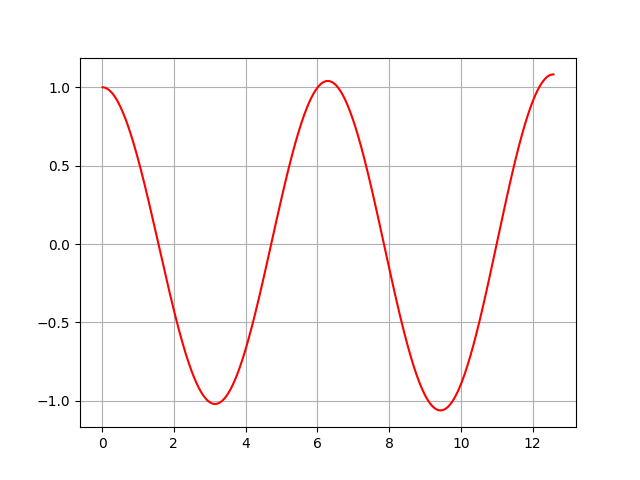
\includegraphics[scale=0.5]{position.png}
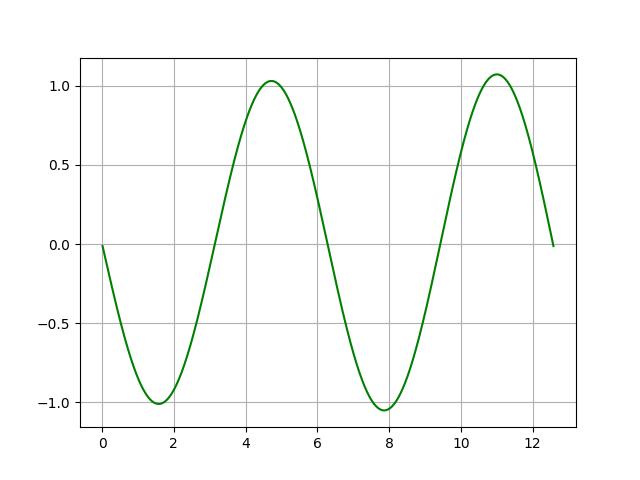
\includegraphics[scale=0.5]{vitesse.png}\\
Le premier graphique correspond à la position $u$ en fonction du temps $t$ et le second graphique correcpond à la vitesse $v$ en fonction du temps $t$.
\begin{center}
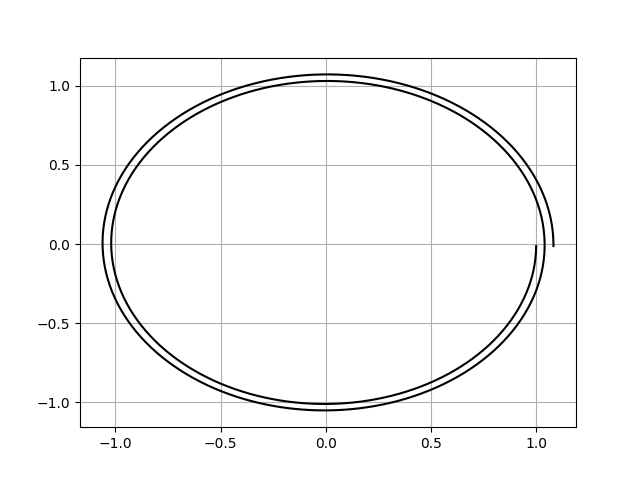
\includegraphics[scale=0.5]{vitpos.png} \\
\end{center}
Ici on à la vitesse $v$ en fonction de la position $u$
On devrais avoir un cercle mais le cercle ne se ferme pas car il y a l'erreur qui est pris en compte. c'est pour cela qu'il y a un décalage sur le graphique.


\end{document}
